\documentclass[10pt]{article}

\usepackage{titlesec}

% Section titles and subsection titles settings
\titleformat{\section}{\normalfont\large\bfseries}{\thesection}{2em}{}
\titlespacing*{\section}{2pt}{*1}{*1}
\titleformat{\subsection}{\normalfont\small\bfseries}{\thesubsection}{1em}{}[]
\titlespacing{\subsection}{0pt}{0.6\baselineskip}{0.6\baselineskip}

% Font
\usepackage{fontspec}
\setmainfont{Arial}

% Page layout
\usepackage[a4paper,margin=0.75in]{geometry}

% Math
\usepackage{mathptmx}  

% Fonts
\usepackage{fontspec}

% Hyperlinks
\usepackage{hyperref}

% Colors
\usepackage{xcolor}

% Tables
\usepackage{booktabs}

% Figures
\usepackage{graphicx}
\usepackage{caption}
\captionsetup[figure]{skip=2pt} 



% Title and Author information
\title{
    \vspace{-2cm}Classification Model Generalization on NinaPro Dataset
}
\author{
    \vspace{0.2cm}Antea Ceko, Chiara Billi, Irene Vardabasso, Ludek Cizinsky, Lou Houngbedji \\
    \vspace{0.2cm} \normalsize{Ecole Polytechnique Fédérale de Lausanne, Switzerland}
}

\date{\today}

\begin{document}
\maketitle

\section{Introduction}
In recent years, Machine Learning based approaches have seen success in many fields, including the medical field.
In this project, we aim to assess various classification models that can predict the type of movement performed by a patient based on the EMG signals recorded from the patient's forearm.
The dataset used for this project is the NinaPro dataset DB1 \cite{ninapro}, which contains EMG signals recorded from 27 patients performing different hand movements. 

\section{Dataset and Preprocessing Steps}
\subsection{General Information}
The surface electromyography (sEMG) data were captured with 10 electrodes, comprising 10 repetitions of 52 distinct movements. 
Participants viewed video prompts on a laptop screen and replicated the movements. Each repetition took 5 seconds, followed by a 3-second rest \cite{ninapro}.
The experiment encompassed three exercise categories: \textbf{1)} fundamental finger movements, \textbf{2)} isometric and isotonic hand configurations, along with basic wrist motions, and \textbf{3)} grasping and functional movements.
% TODO: possibly add the table about the participants


\subsection{Preprocessing}
For the purposes of our work, we decided to focus on the first category of movements, which includes 12 different movements and in total consists of $7.58$ hours of EMG signal data. 
Importantly, the alignment between the EMG signals and corresponding labels has already been done by the authors of the NinaPro dataset. Further, in addressing discrepancies between subject movements and software stimuli, 
the authors applied a generalized likelihood ratio algorithm to correct erroneous movement labels \cite{ninapro}. 
Importantly, the EMG signals were already preprocessed by the manufacturer of the electrodes,
using a Root Mean Square (RMS) filter. This motivated our choice to apply low-pass filtering to the sEMG signals at a cutoff frequency of $5 Hz$ using a zero-phase second-order Butterworth filter
similarly as Atzori et al \cite{ninapro}. 

% Include the preprocessing figure
\begin{figure}[h]
    \centering
    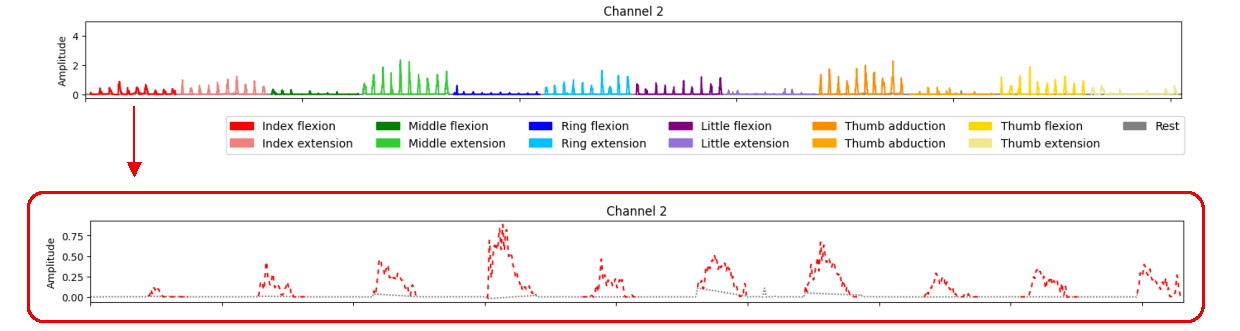
\includegraphics[width=1\textwidth]{../figures/preprocessing.pdf}
    \caption{First plot shows preprocessed EMG signal for the first subject for one of the 10 channels. The subsequent plot facilitates a closer look 
    at the \texttt{Index flexion} finger movement and the 10 repetitions. }
    \label{fig:preprocessing}
\end{figure}

\subsection{Data splitingg}
As the \ref{fig:preprocessing} shows, the EMG signals are recorded in 10 repetitions. Importantly,
there is a variation in amplitude of the EMG signals across the repetitions. Therefore, when spliting the data into training, validation and test sets, 
we made sure that each split is assigned with repetition from both the start and the end of the trial. Specifically,
we assigned the train split to the 1st, 3rd, 5th, 7th and 9th repetitions, the validation split to the 2nd, 4th and 8th repetitions, and the test split to the 6th and 10th repetitions.
This way, we ensured the model is trained and evaluated on the representative data. Notably, since each repetition of a given stimuli is associated with the rest period,
we assigned the rest period to the same split as the corresponding repetition.

Next, for each split and subject, we perfomed windowing with a window size of $500$ ms and a stride of $100$ ms. The chosen window size
allows to capture enough information about the movement to be able to classify it, while the chosen stride allows to capture the temporal dynamics of the movement and 
is a compromise between the computational cost and the amount of information captured. In addition, given data the sampling frequency of $100$ Hz, the chosen step size
means we get a sample for every time point. Importantly, the label for each window is assigned based on the majority label.

\begin{figure}[h]
    \centering
    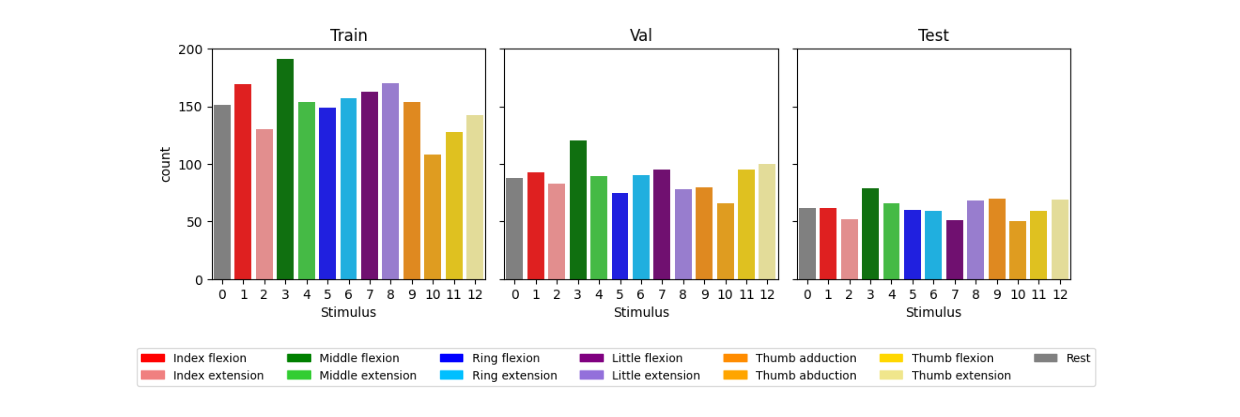
\includegraphics[width=1\textwidth]{../figures/downsampling.pdf}
    \caption{Distribution of the stimuli classes accross splits for the 17th subject.}
    \label{fig:downsampling}
\end{figure}

This windowing approach results in a significant class imbalance between stimuli classes (in total 40 \%) and the rest period (in total 60 \%).
Therefore, we decided to downsample the rest period to the average number of samples per class. This way, we ensured that the model is not biased towards the rest period.

\subsection{Feature Extraction}
For each window, we decided to extract both time and frequency domain features. For time, we extracted 
Mean Absolute Value (\texttt{MAV}), Maximum Absolute Value (\texttt{MaxAV}), Wavelength (\texttt{WL}), Standard Deviation (\texttt{STD}), and Root Mean Square (\texttt{RMS}). 
Additional, in the frequency domain, we considered Mean Power, Total Power, Mean Frequency, Median Frequency, and Peak Frequency. 

\begin{figure}[h]
    \centering
    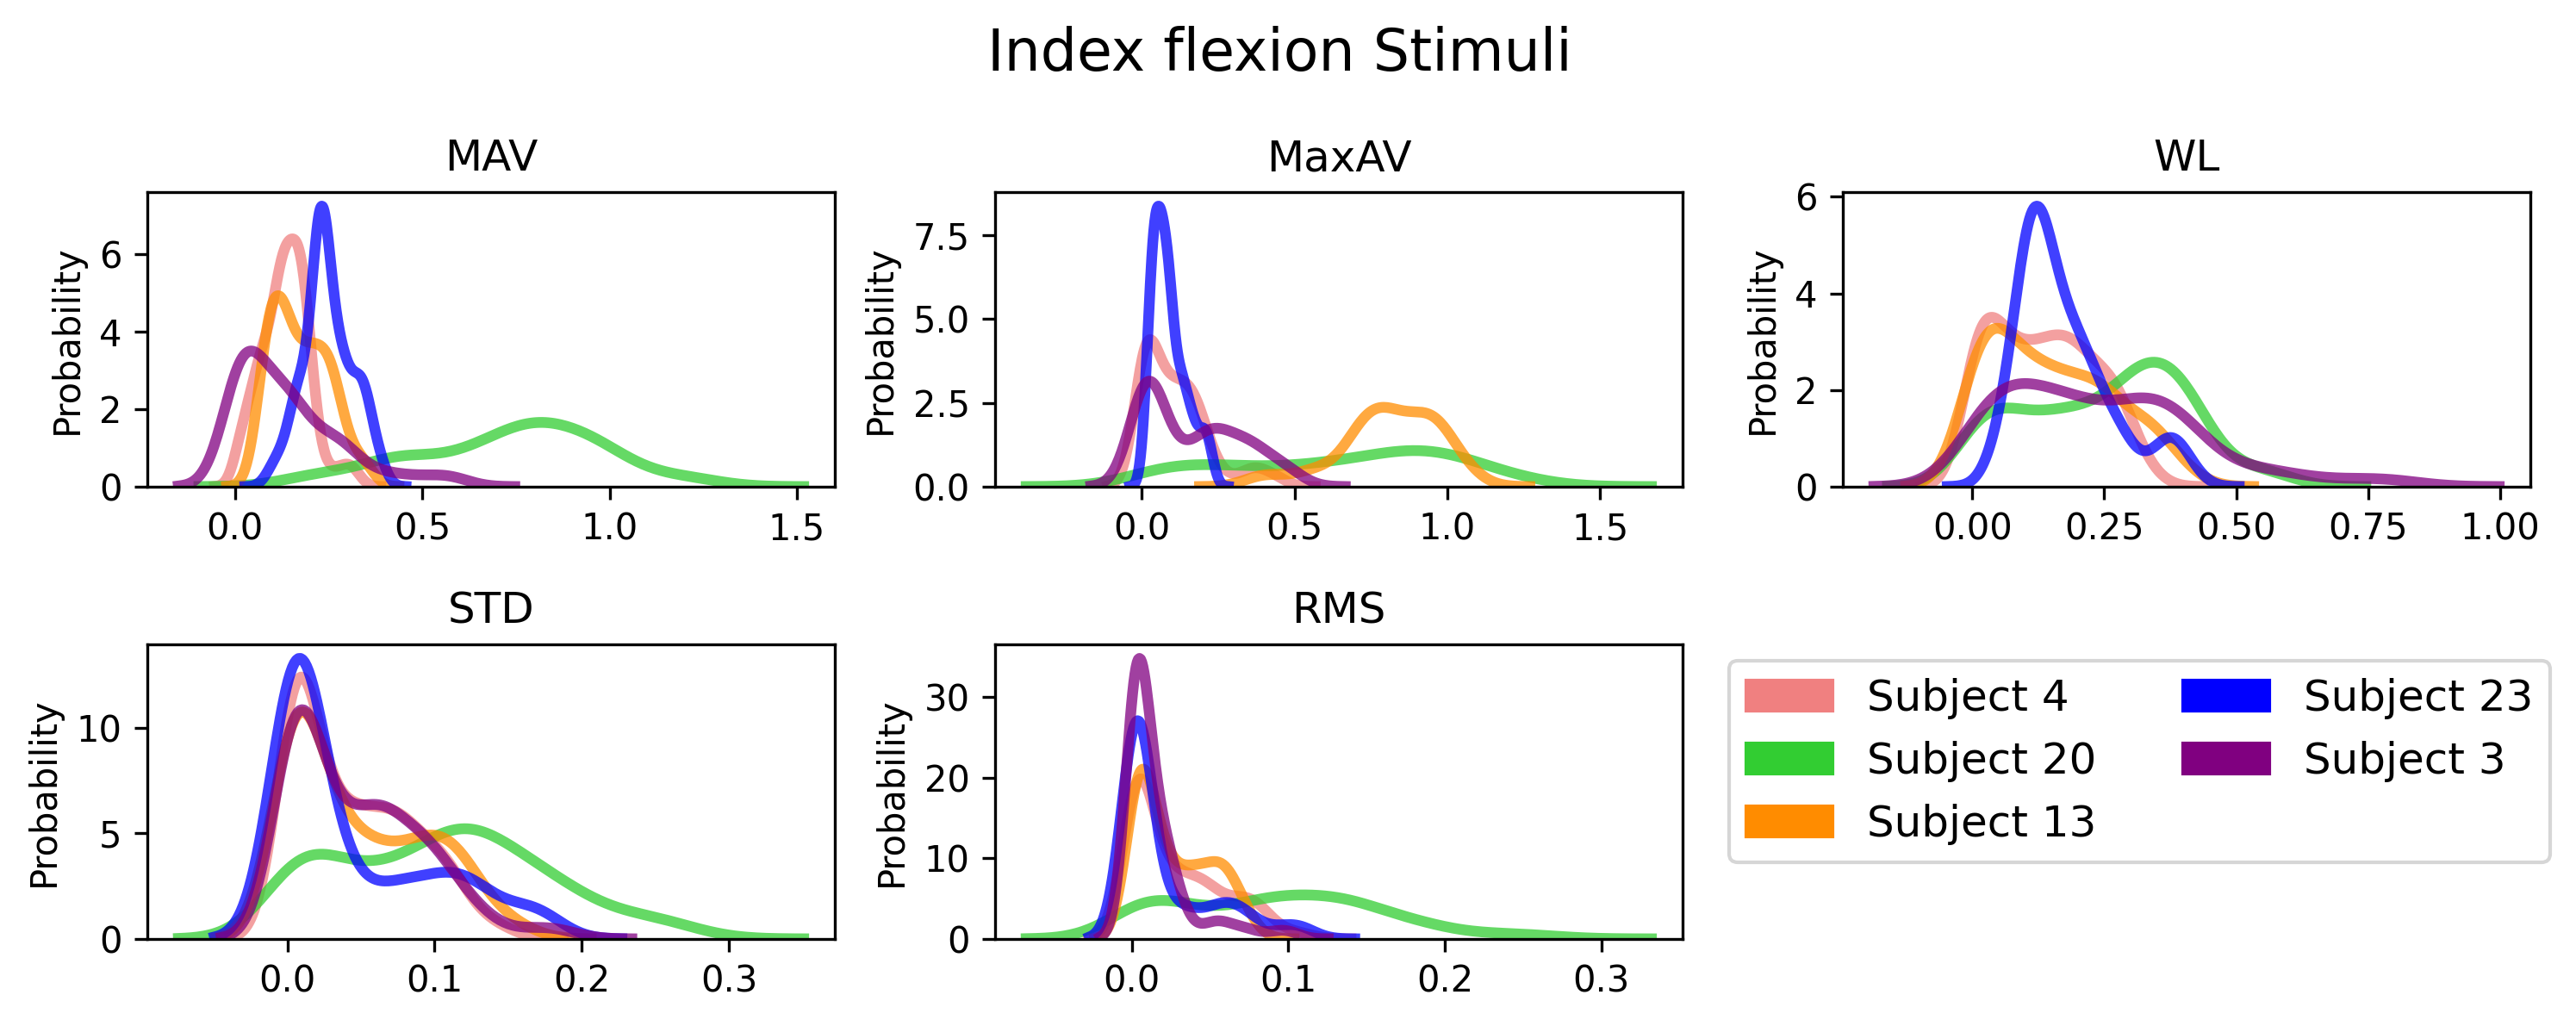
\includegraphics[width=1\textwidth]{../figures/features/time/kde/Index flexion.png}
    \caption{KDE plot estimates for distribution of time features for randomly chosen 5 subjects for \texttt{Index Flexion}.}
    \label{fig:featext}
\end{figure}

% TODO: perhaps would be better if we gave more precise answer to why these difference occur
As the kde plots in figure \ref{fig:featext} suggests, the extracted time features for the chosen stimuli slightly differ accorss subjects.
These could be possibly explained via variations in physiological factors, such as muscle strength, anatomy, or motor control strategies.

\section{Methods}
We start with training and evaluating chosen class of models on individual subjects. This experiment should 
confirm our base hypothesis that the chosen models are capable of generating from given subject's training data to the corresponding validation data.
In addition, we will assess whether the models trained on individual subjects use similar features. Finally, we will find set of hyper-parameters for each
model and evaluate its peformance on the test data of the corresponding subject. In the second part of our experiment, we will choose the best performing model and train it on the selected 
subset of subjects. Finally, we will evaluate its performance on data of subjects which were not seen during training phase. In addition,
we will vary the number of subjects in training dataset to see the impact on model's generalization ability.


\section{Results}
\begin{table}[!ht]
    \centering
    \begin{tabular}{lrrrr}
        \toprule
        \textbf{model} & \textbf{Val Acc} & \textbf{CI} & \textbf{Test Acc} & \textbf{CI} \\
        \midrule
        Random Forest & 0.939 & 0.008 & 0.816 & 0.037 \\
        Logistic Regression & 0.798 & 0.029 & 0.739 & 0.045 \\
        K-Nearest Neighbors & 0.831 & 0.021 & 0.654 & 0.051 \\
        \bottomrule
    \end{tabular}
    \caption{Results of the first experiment.}
    \label{tab:results1}
\end{table}

Here we will describe the results of our experiments. % TODO: need to second table with the results of the second experiment

\section{Discussion}
And here we will discuss the results of our experiments.

\newpage
\bibliographystyle{abbrv}
\bibliography{references}

\end{document}